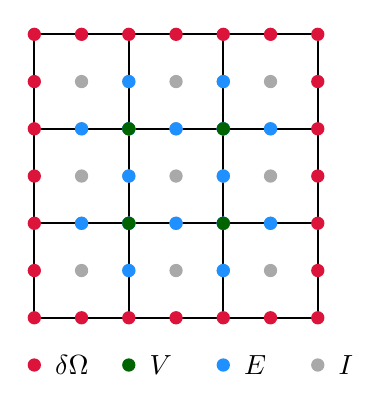
\begin{tikzpicture}[scale=1.2]

    % Colors
    \definecolor{globaledge}{RGB}{220,20,60} % crimson
    \definecolor{vertex}{RGB}{0,100,0} % dark green
    \definecolor{edge}{RGB}{30,144,255} % dodger blue
    \definecolor{interior}{RGB}{169,169,169} % dark gray
    
    % Draw the global square domain
    \draw[thick] (0,0) rectangle (3,3);
    
    % Draw vertical and horizontal grid lines
    \foreach \x in {1,2} {
        \draw[thick] (\x,0) -- (\x,3);
        \draw[thick] (0,\x) -- (3,\x);
    }
    
    % Place the 7x7 nodes
    \foreach \i in {0,...,6} {
        \foreach \j in {0,...,6} {
            % Compute position
            \pgfmathsetmacro{\x}{\i*0.5}
            \pgfmathsetmacro{\y}{\j*0.5}
    

        % Determine node type
        % Global edge (corners and boundary)
        \ifdim\x pt=0pt
            \fill[globaledge] (\x,\y) circle (2pt);
        \else\ifdim\x pt=3pt
            \fill[globaledge] (\x,\y) circle (2pt);
        \else\ifdim\y pt=0pt
            \fill[globaledge] (\x,\y) circle (2pt);
        \else\ifdim\y pt=3pt
            \fill[globaledge] (\x,\y) circle (2pt);
        \else
            % Interior node (not on boundary)
            \fill[interior] (\x,\y) circle (2pt);

            % Edge nodes (on subdomain boundaries)
            \ifdim\x pt=1pt
                \fill[edge] (\x,\y) circle (2pt);
            \else\ifdim\x pt=2pt
                \fill[edge] (\x,\y) circle (2pt);
            \fi\fi
            \ifdim\y pt=1pt
                \fill[edge] (\x,\y) circle (2pt);
            \else\ifdim\y pt=2pt
                \fill[edge] (\x,\y) circle (2pt);
            \fi\fi

            % Vertex nodes (shared by four subdomains)
            \ifdim\x pt=1pt
                \ifdim\y pt=1pt
                    \fill[vertex] (\x,\y) circle (2pt);
                \fi
                \ifdim\y pt=2pt
                    \fill[vertex] (\x,\y) circle (2pt);
                \fi
            \fi
            \ifdim\x pt=2pt
                \ifdim\y pt=1pt
                    \fill[vertex] (\x,\y) circle (2pt);
                \fi
                \ifdim\y pt=2pt
                    \fill[vertex] (\x,\y) circle (2pt);
                \fi
            \fi
        \fi\fi\fi\fi

        }
    }
    
    % Global edge
    \fill[globaledge] (0,-0.5) circle (2pt);
    \node[right=4pt] at (0,-0.5) {$\delta \Omega$};

    % Vertex
    \fill[vertex] (1,-0.5) circle (2pt);
    \node[right=4pt] at (1,-0.5) {$V$};

    % Edge
    \fill[edge] (2,-0.5) circle (2pt);
    \node[right=4pt] at (2,-0.5) {$E$};

    % Interior
    \fill[interior] (3,-0.5) circle (2pt);
    \node[right=4pt] at (3,-0.5) {$I$};

    \end{tikzpicture}